\documentclass{article}
\usepackage{graphicx}
\usepackage[utf8]{inputenc}
\usepackage{amsmath}
\usepackage{amssymb}
\usepackage{graphicx}
\usepackage{epstopdf}
\usepackage{inputenc}
\usepackage{latexsym}
\usepackage{setspace}
\usepackage{caption}
\usepackage{authblk}
\usepackage{float}
\setlength\parindent{24pt}
\usepackage[export]{adjustbox}
\usepackage{wrapfig}
\usepackage{subfig}



\begin{document}

\title{Photoluminescence Spectroscopy of Semiconductors}
\author{Loïc James McKeever}
\affil{Mackenzie Levangie}

\maketitle

\section{Introduction}

The objective of this lab is to study spectrographic data from a variety of sources; ambient room light and the luminescence of several semiconductor samples.  Using this data we can gain information about various properties of these samples.  We can determine the elemental composition of the light source in the room and of certain alloys and the diameter of nanoparticles.  Here we determined that the lights in the room most likely used mercury vapor fluorescence.  The concentration of gallium in our sample of $InGaP$ was determined to be $0.614_{-0.268}^{+0.262}$.  The diameter of our $CdTe$ nanoparticles was found to be $2.75 \pm 0.24$ nm.

\section{Materials and Methods}

In this experiment we will study the fluorescence of a variety of samples; $GaAs$, $InP$, $Ga_{1-x}In_{x}P$ alloy with unknown $x$ and $CdTe$ nanoparticles of unknown size. When a material is hit by light at certain frequencies that light can excited electrons of the valence band to higher energy states.  These electrons then descend to the conduction band via non-radiative relaxation means.  They then return to the valence band by emitting a photon(photoluminescence) with energy equivalent to the difference between the valence band and the conduction band.  See Figure 1 (a).  This is called the band gap energy.  The band gap energy depends on a variety of things such as the elemental composition or even the temperature. 

\begin{figure}%
   \centering
    \subfloat[This figure describes the process by which photoluminescence originates.]{{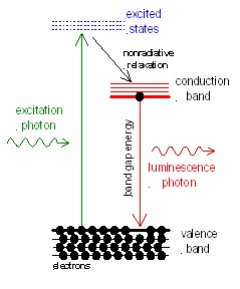
\includegraphics[scale=0.8]{photoluminescence.PNG} }}%
    \qquad
    \subfloat[Diagram of optical setup used to gather data from our semiconductor samples.]{{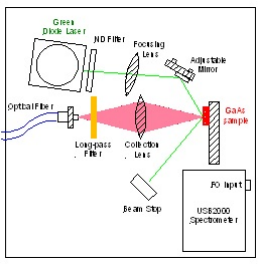
\includegraphics[scale=0.8]{SetUp.PNG} }}%
    \caption{Diagrams describing fluorescence and the optical setup used to measure it in this lab.$^{[1]}$}%
    \label{fig:example}%
\end{figure}

Using the optical setup described in Figure 1 (b) we were able to gather spectral data from these samples.  The data was gathered using an USB2000-FLG Ocean Optics spectrometer which was connected to our computer via USB cable and OceanOptics OOIBase32 software was used to read and save the data.  The data was then analyzed using various Matlab scripts written ourselves. 

\section{Results}

We started by taking the spectral data of the ambient light in the room.  See Figure 2. 

\begin{figure}[H]
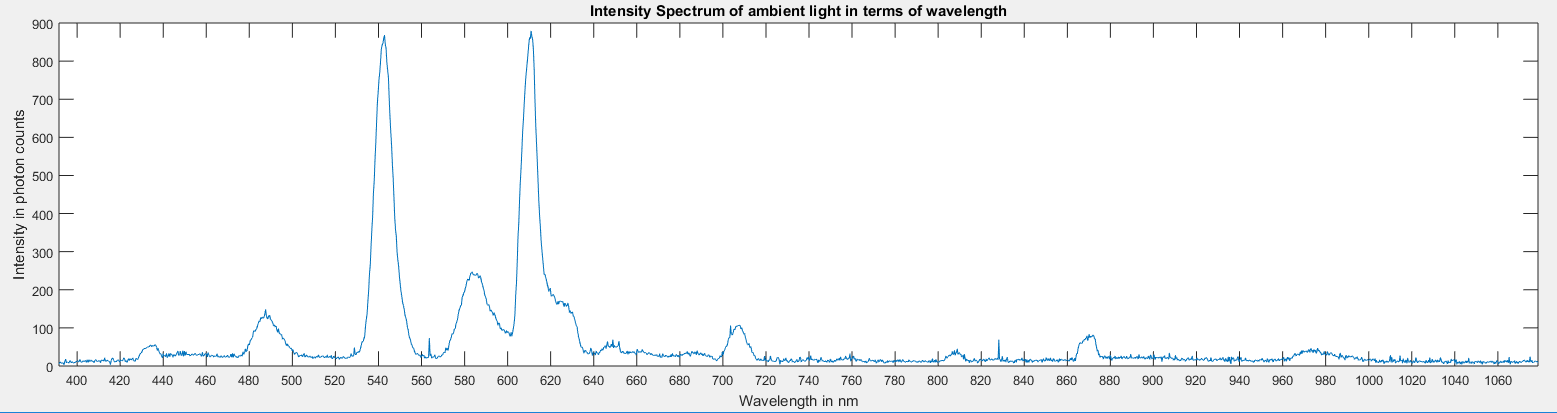
\includegraphics[scale=.5,center]{RoomSpec.PNG}
\caption{Spectral data of the ambient light of the room.  Integration time was 0.2 seconds and the Full Width Half Maximum(FWHM) of the thinnest peak is 8.585 nm.}
\end{figure}

From there we were able to determine the positions of the six largest peaks using our Matlab code.

\begin {table}[H]
\begin{center}
 \begin{tabular}{|c | c| c|} 
 \hline
 Wavelength(in nm) & Intensity(in counts per second)  & Corresponding Element\\ [1ex] 
 \hline\hline
 610.91 & 4396.7 & Mercury\\ 
 \hline
 542.80 & 4341.7 & Mercury\\
 \hline
 583.59 & 1236.7 & Mercury\\
 \hline
 489.43 & 666.67 & Mercury\\
 \hline
 707.35 & 536.67 & Mercury\\ 
 \hline
 870.09 & 416.67 & Mercury \\
 \hline
\end{tabular}
\end{center}
\caption {Six main peaks from the ambient room light spectrum, their wavelengths and the element to which they most likely correspond to (within error).} \label{tab:title}
\end{table}

\begin{figure}[H]

\includegraphics[scale=.5,center]{mercury.jpg}
\caption{Mercury emission spectrum.$^{[2]}$  Source also included quantitative data.}
\end{figure}

Next we aimed the laser at out $GaAs$ sample to collect the spectral data from its fluorescence.  We analyzed the data in Matlab to get the FWHM(and thus the error) of the main peak in both nanometers and meV.  See Figures 4 and 5.

\begin{figure}[H]
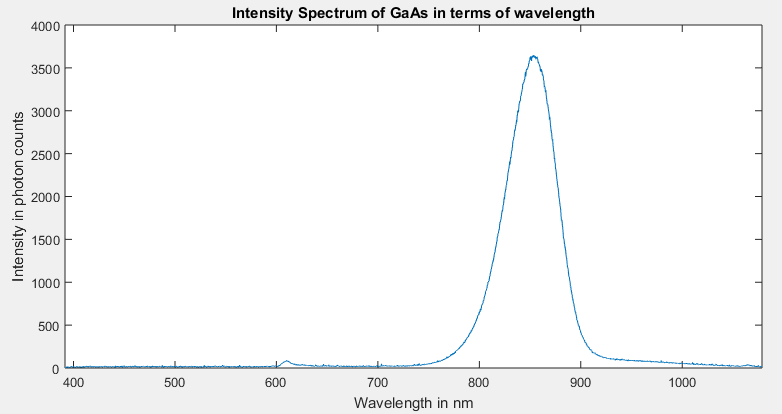
\includegraphics[scale=.65,center]{GaAsNm.PNG}
\caption{Spectral data of the $GaAs$ fluorescence in terms of wavelength.  Integration time was 0.2 seconds.  The peak is located at 853.11 nm and the FWHM of the peak is 57.95 nm which means we have an error of 24.61 nm.  Assuming a Gaussian distribution and $\sigma=\frac{FWHM}{2.355}.$}
\end{figure}

\begin{figure}[H]
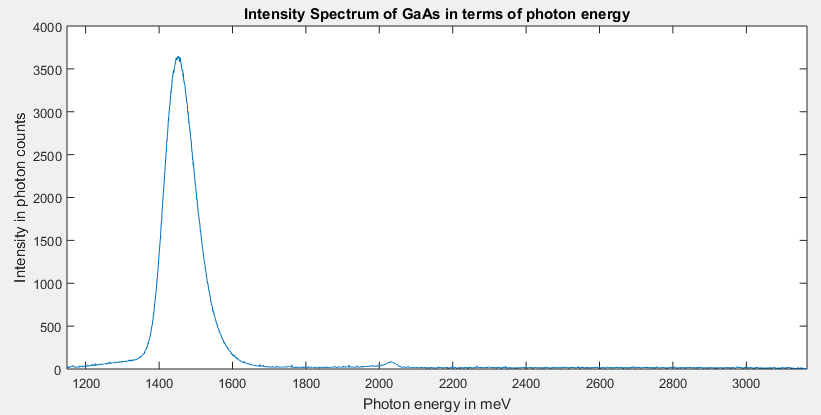
\includegraphics[scale=.65,center]{GaAsEv.PNG}
\caption{Spectral data of the $GaAs$ fluorescence in terms of photon energy.  Integration time was 0.2 seconds.  The peak is located at 1452.9 meV and the FWHM of the peak is 99.21 meV which means we have an error of 42.13 meV.}
\end{figure}

The same was done with the $InP$ and the $InGaP$ samples next.  See Figures 6 and 7.

\begin{figure}[H]
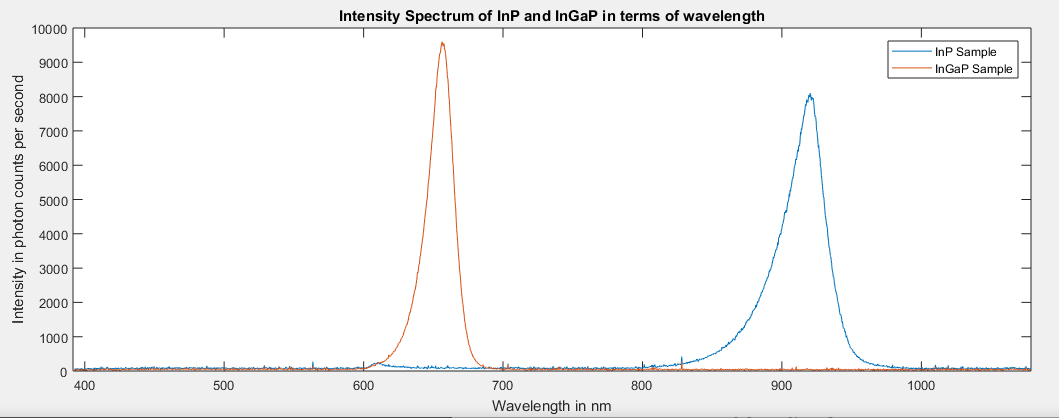
\includegraphics[scale=.7,center]{ingapnm.PNG}
\caption{Spectral data of the $InP$ and $InGaP$ fluorescence in terms of wavelength.  Integration time was 0.2 seconds for the $InP$ and 0.3 seconds for the $InGaP$ so the data was normalized for both to counts per second.  The $InP$ peak is located at 920.20 nm and the FWHM of the peak is 33.34 nm which means we have an error of 14.16 nm.  The $InGaP$ peak is located at 656.27 nm and the FWHM of the peak is 21.02 nm which means we have an error of 8.92 nm.}
\end{figure}

\begin{figure}[H]
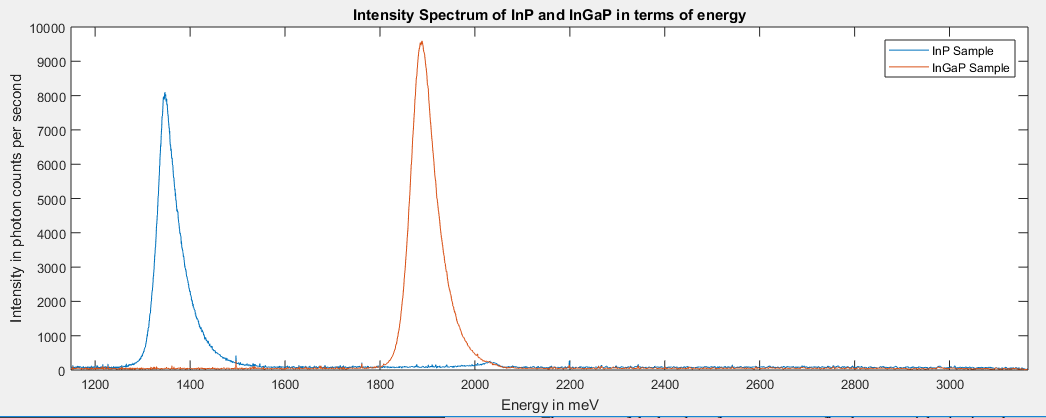
\includegraphics[scale=.7,center]{ingapev.PNG}
\caption{Spectral data of the $InP$ and $InGaP$ fluorescence in terms of photon energy.  The $InP$ peak is located at 1347.0 meV and the FWHM of the peak is 49.26 meV which means we have an error of 20.92 meV.  The $InGaP$ peak is located at 1888.7 meV and the FWHM of the peak is 60.66 meV which means we have an error of 25.76 meV.}
\end{figure}

This peak corresponds to the bandgap energy between two energy states.  The photon is emitted as an electron goes from an excited state to a relaxed state.  The bandgap energy can be changed by alloying, by substituting $Ga$ for $In$. The bandgap of the alloy $In_{1-x}Ga_{x}P$ has an polynomial energy dependence given by the following equation

\begin{equation}
    E(x)=E_o + 512x + 603x^2
\end{equation}

where $E$ is the band gap of the alloy, $E_o$ is the bandgap of $InP$ and $x$ is the concentration of $Ga$.  The units here are meV.  With the values we found we calculate a gallium concentration of 0.614 with an uncertainty range of 0.5872 to 0.6402.  From Equation 1 we can determine the required concentration of $Ga$ to shift the bandgap into the orange region(590 nm) and it is 0.77. 

Finally the same was done with the sample of $CdTe$ nanoparticles.  See Figures 8 and 9.

\begin{figure}[H]
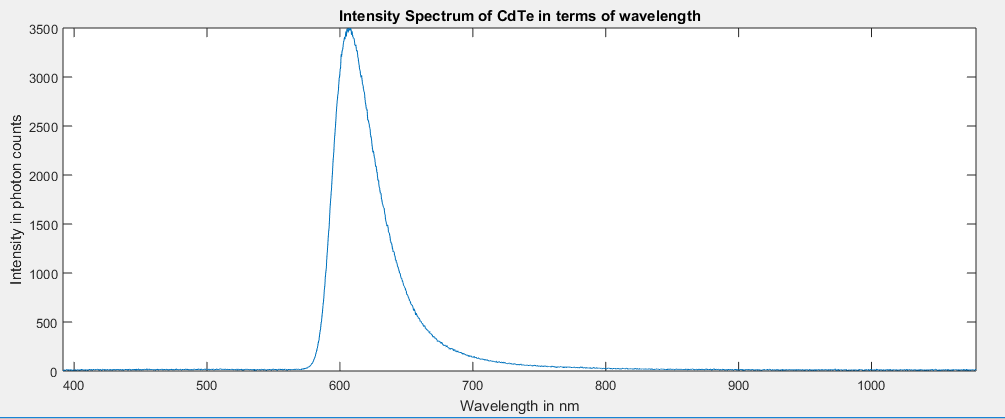
\includegraphics[scale=.65,center]{cdtenm.PNG}
\caption{Spectral data of the $CdTe$ nanoparticle fluorescence in terms of wavelength.  Integration time was 3 milliseconds.  The peak is located at 606.62 nm and the FWHM of the peak is 38.42 nm which means we have an error of 16.31 nm.}
\end{figure}

\begin{figure}[H]
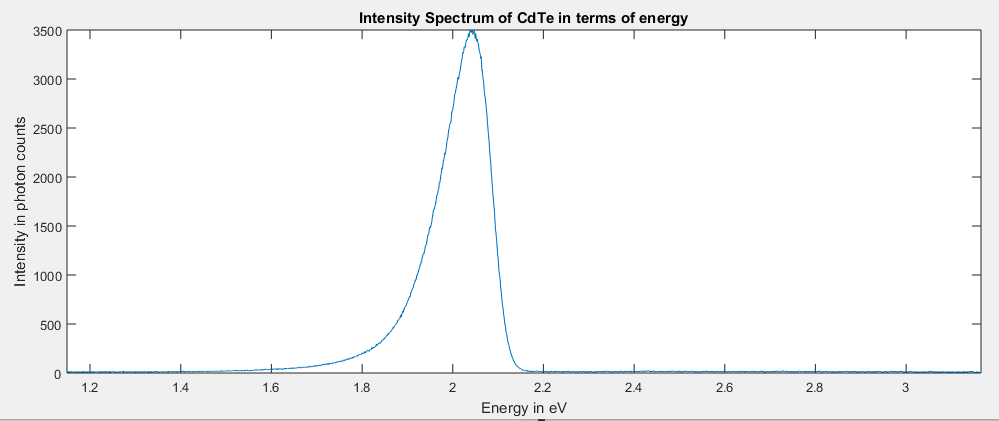
\includegraphics[scale=.65,center]{cdteev.PNG}
\caption{Spectral data of the $CdTe$ nanoparticle fluorescence in terms of photon energy.  Integration time was 0.2 seconds.  The peak is located at 2.04 eV and the FWHM of the peak is 0.13 eV which means we have an error of 0.054 eV.}
\end{figure}

The bandgap energy can also change based on the size of the particles.  When the particles are less than 100 nm they experience "quantum confinement" and the change in the bandgap is given by the following equation

\begin{equation}
    E_{NP}=E_o+\frac{\hbar^2k^2}{2m}
\end{equation}

where $E_o$ is the bandgap of CdTe that aren't experiencing quantum confinement, $k=\frac{\pi}{d}$ is the wavevector, $m$ is the effective mass of the excited electron and $d$ is the diameter of the nanoparticle.  This gives us therefore

\begin{equation}
    E_{NP}=E_o+\frac{\hbar^2\pi^2}{2md^2}
\end{equation}

Here we'll use $E_o=1.49 eV$ and $m=0.9m_o$ where $m_o=5.6856*10^{-12} eV$ is the mass of a free electron.  From Equation 3 we find the diameter of the CdTe nanoparticles to be 2.75 $\pm$ 0.24 nm.

\section{Discussion}

Most modern fluorescent bulbs use mercury vapor so it makes sense that the light in a room with those bulbs would be found to have the composition we found in our first result.

We know that to shift the band gap of $InP$ from 920 nm to red light(700 nm) you need a concentration of gallium of 0.55 and we determined the to shift to the orange region(590 nm) you a concentration of 0.77.  So given that the main peak of our $InGaP$ sample was found to be at 656.27 $\pm$ 8.92 nm, which is right in the middle of the red and orange regions, the concentration range of 0.5872 to 0.6402 we found is completely consistent with what we'd expect.

Finally $CdTe$ nanoparticles of our sample were found to be 2.75 $\pm$ 0.24 nm in diameter.  $CdTe$ can vary in size depending on how they were synthesized but generally they're less than 10 nm$^{[3]}$ so our results are consistent with what we'd expect of only a few nanometers.

\section{Conclusions}

In conclusion we determined that the ambient light in the room was most likely from mercury fluorescence which is consistent with most modern fluorescence bulbs that use mercury vapor.  The concentration of gallium in our $InGaP$ sample was found to be between 0.5872 and 0.6402 nm which is consisten with what we'd expect given a shift in the emission peak to between the red and orange regions.  Finally the sample of $CdTe$ was found to have nanoparticles of 2.75 $\pm$ 0.24 nm in diameter which is consistent with what we'd expect of only a few nanometers.

\section{References}

[1] Photoluminescence Spectroscopy of Semiconductors Lab Manual, Northeastern University

\noindent [2] Spectra of Gas Discharges, Joachim Köppen Strasbourg, Illkirch, Kiel 2007 

\noindent [3] CdTe Nanoparticles and Clusters, A. D. Styrkas, Institute of Solid State Physics, Russian Academy of Sciences, 2007

\section{Appendix}

See code attached.  

\noindent fwhm function written by Patrick Egan in 2006

\end{document}
